\subsection*{Zestaw XXVI --- Rachunek różniczkowy (zadania otwarte)}
\subsubsection*{Zadanie~1.}
\begin{equation*}
    f\pars{x} = x + 4 + \frac{4}{x} \qquad x \in \open{0}{+\infty}
\end{equation*}
Obliczmy pochodną tej funkcji:
\begin{equation*}
    f'\pars{x}
        = 1 - \frac{4}{x^2}
        = \frac{x^2 - 4}{x^2}
        = \frac{\pars{x + 2}\pars{x - 2}}{x^2}
\end{equation*}
Mianownik jest zawsze dodatni, więc znak pochodnej zależy tylko od licznika. Zatem wykres znaku pochodnej wygląda następująco:
\begin{equation*}
    \upparabola{-2}{2}
\end{equation*}
Interesuje nas tylko przedział \(\open{0}{+\infty}\). W~przedziale \(\open{0}{2}\) pochodna jest ujemna, dla \(x = 2\) przyjmuje wartość \(0\), a~w~przedziale \(\open{2}{+\infty}\) jest dodatnia. Oznacza to, że funkcja \(f\) jest malejąca w~przedziale \(\open{0}{2}\) i~rosnąca w~przedziale \(\open{2}{+\infty}\), więc dla \(x = 2\) przyjmuje globalną wartość najmniejszą:
\begin{equation*}
    S_\p{min} = S\pars{2} = 2 + 4 + \frac{4}{2} = 8
\end{equation*}
Zatem najmniejszą wartością przyjmowaną przez tę funkcję jest \(8\).
\qed
\subsubsection*{Zadanie~2.}
\begin{equation*}
    f\pars{x} = \frac{1}{x^3} + 2x \qquad x \in \real \setminus \set{0}
\end{equation*}
Obliczmy pochodną tej funkcji, aby móc wyznaczyć współczynnik kierunkowy stycznej:
\begin{equation*}
    f'\pars{x} = -\frac{3}{x^4} + 2
\end{equation*}
Zatem współczynnik kierunkowy prostej stycznej do wykresu \(y = f\pars{x}\) wystawionej w~punkcie \(x_0 = -1\) wynosi
\begin{equation*}
    f'\pars{-1}
        = -\frac{3}{\pars{-1}^4} + 2
        = -3 + 2
        = -1
\end{equation*}
Teraz musimy tylko dokonać odpowiedniej translacji tej prostej, aby przechodziła przez punkt \(\pars{x_0; f\pars{x_0}}\):
\begin{equation*}
    y
        = f'\pars{-1}\pars{x - \pars{-1}} + f\pars{-1}
        = -1\pars{x + 1} + \frac{1}{\pars{-1}^3} + 2 \cdot \pars{-1}
        = -x - 1 - 1 - 2
        = -x - 4
\end{equation*}
Zatem prosta styczna do wykresu \(y = f\pars{x}\) wystawiona w~punkcie \(x_0 = -1\) ma równanie
\begin{equation*}
    y = -x - 4
\end{equation*}
\subsubsection*{Zadanie~3.}
\begin{equation*}
    f\pars{x} = 4x + \frac{9}{x} \qquad x \in \real \setminus \set{0}
\end{equation*}
Obliczmy pochodną tej funkcji, aby zbadać monotoniczność i~ekstrema:
\begin{equation*}
    f'\pars{x}
        = 4 - \frac{9}{x^2}
        = \frac{4x^2 - 9}{x^2}
        = \frac{\pars{2x + 3}\pars{2x - 3}}{x^2}
\end{equation*}
Mianownik jest zawsze dodatni, więc znak pochodnej zależy tylko od licznika. Dlatego wykres znaku pochodnej wygląda następująco:
\begin{gather*}
    \upparabola{-\frac{3}{2}}{\frac{3}{2}}\\
    \tag{\(1\)} \forall x \in \open{-\infty}{-\frac{3}{2}}\colon f'\pars{x} > 0 \label{2020_11_06:3:first_increase}\\
    \tag{\(2\)} f'\pars{-\frac{3}{2}} = 0 \label{2020_11_06:3:first_zero}\\
    \tag{\(3\)} \forall x \in \open{-\frac{3}{2}}{\frac{3}{2}}\colon f'\pars{x} < 0 \label{2020_11_06:3:decrease}\\
    \tag{\(4\)} f'\pars{\frac{3}{2}} = 0 \label{2020_11_06:3:second_zero}\\
    \tag{\(5\)} \forall x \in \open{\frac{3}{2}} f'\pars{x} > 0 \label{2020_11_06:3:second_increase}
\end{gather*}
Oznacza to, że
\begin{description}
    \item \(\mbox{(\ref{2020_11_06:3:first_increase})} \implies\) funkcja \(f\) jest rosnąca w~przedziale \(\open{-\infty}{-\frac{3}{2}}\)
    \item \(\mbox{(\ref{2020_11_06:3:first_increase})} \land \mbox{(\ref{2020_11_06:3:first_zero})} \land \mbox{(\ref{2020_11_06:3:decrease})} \implies\) funkcja \(f\) przyjmuje dla \(x = -\frac{3}{2}\) maksimum lokalne:
        \begin{equation*}
            f\pars{-\frac{3}{2}}
                = 4 \cdot \pars{-\frac{3}{2}} + \frac{9}{-\frac{3}{2}}
                = -6 + \pars{-6}
                = -12
        \end{equation*}
    \item \(\mbox{(\ref{2020_11_06:3:decrease})} \implies\) funkcja \(f\) jest malejąca w~przedziale \(\open{-\frac{3}{2}}{\frac{3}{2}}\)
    \item \(\mbox{(\ref{2020_11_06:3:decrease})} \land \mbox{(\ref{2020_11_06:3:second_zero})} \land \mbox{(\ref{2020_11_06:3:second_increase})} \implies\) funkcja \(f\) przyjmuje dla \(x = \frac{3}{2}\) minimum lokalne:
        \begin{equation*}
            f\pars{\frac{3}{2}}
                = 4 \cdot \frac{3}{2} + \frac{}{9}{\frac{3}{2}}
                = 6 + 6
                = 12
        \end{equation*}
    \item \(\mbox{(\ref{2020_11_06:3:second_increase})} \implies\) funkcja \(f\) jest rosnąca w~przedziale \(\open{\frac{3}{2}}{+\infty}\)
\end{description}
\subsubsection*{Zadanie~4.}
\begin{equation*}
    y\pars{x} = \frac{x^3}{3} + x^2 = \frac{1}{3}x^2\pars{x + 3} \qquad x \in \real
\end{equation*}
Z~postaci iloczynowej odczytujemy, że pierwiastkami są \(x = 0\) oraz \(x = -3\). Obliczmy pochodną tego wyrażenia:
\begin{equation*}
    y'\pars{x} = x^2 + 2x = \pars{x + 2}x
\end{equation*}
Wykres znaku pochodnej:
\begin{gather*}
    \upparabola{-2}{0}\\
    \tag{\(1\)} \forall x \in \open{-\infty}{-2}\colon y'\pars{x} > 0 \label{2020_11_06:4:first_increase}\\
    \tag{\(2\)} y'\pars{-2} = 0 \label{2020_11_06:4:first_zero}\\
    \tag{\(3\)} \forall x \in \open{-2}{0}\colon y'\pars{x} < 0 \label{2020_11_06:4:decrease}\\
    \tag{\(4\)} y'\pars{0} = 0 \label{2020_11_06:4:second_zero}\\
    \tag{\(5\)} \forall x \in \open{0}{+\infty}\colon y'\pars{x} > 0 \label{2020_11_06:4:second_increase}
\end{gather*}
Oznacza to, że
\begin{description}
    \item \(\mbox{(\ref{2020_11_06:4:first_increase})} \implies\) funkcja \(y\) jest rosnąca w~przedziale \(\open{-\infty}{-2}\)
    \item \(\mbox{(\ref{2020_11_06:4:first_increase})} \land \mbox{(\ref{2020_11_06:4:first_zero})} \land \mbox{(\ref{2020_11_06:4:decrease})} \implies\) funkcja \(y\) przyjmuje dla \(x = -2\) maksimum lokalne:
        \begin{equation*}
            y\pars{-2} = \frac{-8}{3} + 4 = \frac{4}{3}
        \end{equation*}
    \item \(\mbox{(\ref{2020_11_06:4:decrease})} \implies\) funkcja \(y\) jest malejąca w~przedziale \(\open{-2}{0}\)
    \item \(\mbox{(\ref{2020_11_06:4:decrease})} \land \mbox{(\ref{2020_11_06:4:second_zero})} \land \mbox{(\ref{2020_11_06:4:second_increase})} \implies\) funkcja \(y\) przyjmuje dla \(x = 0\) minimum lokalne:
        \begin{equation*}
            y\pars{0} = \frac{0}{3} + 0 = 0
        \end{equation*}
    \item \(\mbox{(\ref{2020_11_06:4:second_increase})} \implies\) funkcja \(y\) jest rosnąca w~przedziale \(\open{0}{+\infty}\)
\end{description}
Na podstawie tych informacji możemy naszkicować wykres funkcji \(y\pars{x}\):
\begin{equation*}
    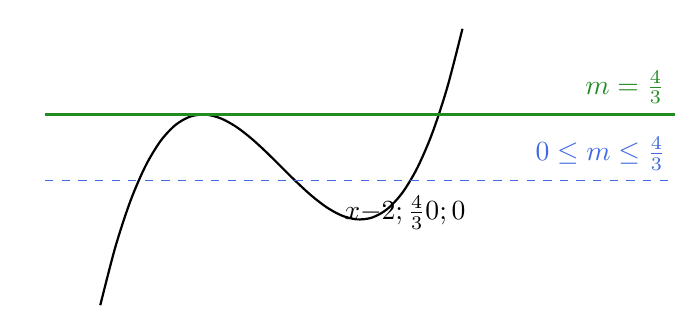
\begin{tikzpicture}
        \drawvec[ForestGreen] (-4, 0) -- (4, 0) node[below]{\(x\)};
        \draw[domain=-3.3:1.3, thick, smooth] plot (\x, {1/3*\x*\x*(\x + 3)});
        \draw[ForestGreen, very thick] (-4, 4/3) -- (4, 4/3) node[above left]{\(m = \frac{4}{3}\)};
        \draw[RoyalBlue, dashed] (-4, 0.5) -- (4, 0.5) node[above left]{\(0 \leq m \leq \frac{4}{3}\)};
        \fillpoint*{-2, 4/3}[\(\pars{-2; \frac{4}{3}}\)][above];
        \fillpoint*{0, 0}[\(\pars{0; 0}\)][below];
    \end{tikzpicture}
\end{equation*}
Z~tego wykresu odczytujemy, że aby prosta \(m\) miała co najmniej dwa punkty wspólne z~wykresem \(y\pars{x}\), musi zachodzić
\begin{equation*}
    m \in \closed{0}{\frac{4}{3}}
\end{equation*}
\subsubsection*{Zadanie~5.}
\begin{gather*}
    f\pars{x} = \frac{x^5}{5} - \frac{16}{3}x^3 \qquad x \in \real\\
    f'\pars{x} = x^4 - 16x^2 = x^2\pars{x^2 - 16} = \pars{x + 4}x^2\pars{x - 4}
\end{gather*}
Współczynnik przy najwyższej potędze w~wielomianie będącym pochodną jest dodatni, więc w~\(+\infty\) pochodna przyjmuje dowolnie duże wartości. Szkic wykresu pochodnej będzie więc wyglądał tak:
\begin{equation*}
    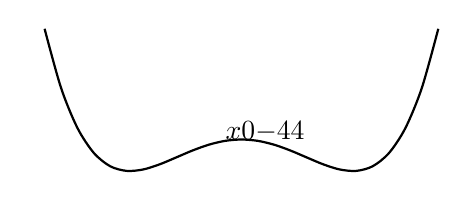
\begin{tikzpicture}
        \drawvec (-4, 0) -- (4, 0) node[below]{\(x\)};
        \draw[domain=-2.5:2.5, thick, smooth] plot (\x, {0.1*\x*\x*(\x - 2)*(\x + 2)});
        \fillpoint*{0, 0}[\(0\)][below];
        \fillpoint*{-2, 0}[\(-4\)][above right];
        \fillpoint*{2, 0}[\(4\)][above left];
    \end{tikzpicture}
\end{equation*}
Odczytujemy z~niego, że
\begin{equation*}
    f'\pars{x} \leq 0 \iff x \in \closed{-4}{4}
\end{equation*}
W~tym przedziale znajduje się \(9\) liczb całkowitych:
\begin{equation*}
    \set{-4, -3, -2, -1, 0, 1, 2, 3, 4}
\end{equation*}
Zatem
\begin{equation*}
    \card{\set{x \in \integer : f'\pars{x} \leq 0}} = 9
\end{equation*}
\subsubsection*{Zadanie~6.}
\begin{equation*}
    y\pars{x} = \frac{1}{2}x^2 \qquad x \in \real
\end{equation*}
Odległość jest zawsze dodatnia, więc uzasadnienie, że pewna odległość jest nie mniejsza niż \(\sqrt{7}\) jest równoważne pokazaniu, że kwadrat tej odległości jest nie mniejszy niż \(7\). Kwadrat odległości w~kartezjańskim układzie współrzędnych możemy obliczyć z~twierdzenia Pitagorasa. Niech \(\pars{x, y\pars{x}}\) oznacza pewien punkt paraboli. Zdefiniujmy funkcję kwadratu odległości takiego punktu od punktu \(M = \pars{0; 4}\) w~zależności od \(x\):
\begin{equation*}
    f\pars{x}
        = \pars{x - 0}^2 + \pars{\frac{1}{2}x^2 - 4}^2
        = x^2 + \frac{1}{4}x^4 - 4x^2 + 16
        = \frac{1}{4}x^4 - 3x^2 + 16
\end{equation*}
Obliczmy pochodną tej funkcji:
\begin{equation*}
    f'\pars{x}
        = x^3 - 6x
        = x\pars{x^2 - 6}
        = \pars{x + \sqrt{6}}x\pars{x - \sqrt{6}}
\end{equation*}
Wykres znaku pochodnej wygląda więc następująco:
\begin{gather*}
    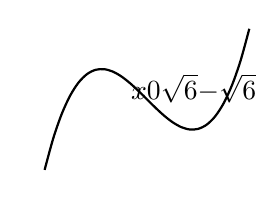
\begin{tikzpicture}
        \drawvec (-2, 0) -- (2, 0) node[below]{\(x\)};
        \draw[domain=-1.3:1.3, thick, smooth] plot (\x, {\x*(\x - 1)*(\x + 1)});
        \fillpoint*{0, 0}[\(0\)][below];
        \fillpoint*{1, 0}[\(\sqrt{6}\)][below right];
        \fillpoint*{-1, 0}[\(-\sqrt{6}\)][above left];
    \end{tikzpicture}\\
    \tag{\(1\)} \forall x \in \open{-\infty}{-\sqrt{6}}\colon f'\pars{x} < 0 \label{2020_11_06:6:first_decrease}\\
    \tag{\(2\)} f'\pars{-\sqrt{6}} = 0 \label{2020_11_06:6:first_zero}\\
    \tag{\(3\)} \forall x \in \open{-\sqrt{6}}{0}\colon f'\pars{x} > 0 \label{2020_11_06:6:first_increase}\\
    \tag{\(4\)} f'\pars{0} = 0 \label{2020_11_06:6:second_zero}\\
    \tag{\(5\)} \forall x \in \open{0}{\sqrt{6}}\colon f'\pars{x} < 0 \label{2020_11_06:6:second_decrease}\\
    \tag{\(6\)} f'\pars{\sqrt{6}} = 0 \label{2020_11_06:6:third_zero}\\
    \tag{\(7\)} \forall x \in \open{\sqrt{6}}{+\infty}\colon f'\pars{x} > 0 \label{2020_11_06:6:second_increase}
\end{gather*}
Oznacza to, że
\begin{description}
    \item \(\mbox{(\ref{2020_11_06:6:first_decrease})} \implies\) funkcja \(f\) jest malejąca w~przedziale \(\open{-\infty}{-\sqrt{6}}\)
    \item \(\mbox{(\ref{2020_11_06:6:first_decrease})} \land \mbox{(\ref{2020_11_06:6:first_zero})} \land \mbox{(\ref{2020_11_06:6:first_increase})} \implies\) funkcja \(f\) osiąga dla \(x = -\sqrt{6}\) minimum lokalne:
        \begin{equation*}
            f\pars{-\sqrt{6}}
                = \frac{1}{4} \cdot 36 - 3 \cdot 6 + 16
                = 9 - 18 + 16
                = 7
        \end{equation*}
    \item \(\mbox{(\ref{2020_11_06:6:first_increase})} \implies\) funkcja \(f\) jest rosnąca w~przedziale \(\open{-\sqrt{6}}{0}\)
    \item \(\mbox{(\ref{2020_11_06:6:first_increase})} \land \mbox{(\ref{2020_11_06:6:second_zero})} \land \mbox{(\ref{2020_11_06:6:second_decrease})} \implies\) funkcja \(f\) osiąga dla \(x = 0\) maksimum lokalne:
        \begin{equation*}
            f\pars{0} = 16
        \end{equation*}
    \item \(\mbox{(\ref{2020_11_06:6:second_decrease})} \implies\) funkcja \(f\) jest malejąca w~przedziale \(\open{0}{\sqrt{6}}\)
    \item \(\mbox{(\ref{2020_11_06:6:second_decrease})} \land \mbox{(\ref{2020_11_06:6:third_zero})} \land \mbox{(\ref{2020_11_06:6:second_increase})} \implies\) funkcja \(f\) osiąga dla \(x = \sqrt{6}\) minimum lokalne:
        \begin{equation*}
            f\pars{\sqrt{6}}
                = \frac{1}{4} \cdot 36 - 3 \cdot 6 + 16
                = 7
        \end{equation*}
    \item \(\mbox{(\ref{2020_11_06:6:second_increase})} \implies\) funkcja \(f\) jest rosnąca w~przedziale \(\open{\sqrt{6}}{+\infty}\)
\end{description}
Zatem wykres funkcji wygląda następująco:
\begin{equation*}
    \begin{tikzpicture}
        \def\rt{\fpeval{sqrt(6)}};
        \drawvec (-4, 0) -- (4, 0) node[below]{\(x\)};
        \draw (-4, 1.4) -- (4, 1.4) node[right]{\(y = 7\)};
        \draw[domain=-4:4, smooth, thick, samples=50] plot (\x, {0.2*(0.25*pow(\x, 4) - 3*pow(\x, 2) + 16)});
        \fillpoint*{0, 3.2}[\(\pars{0, 16}\)][above];
        \fillpoint*{-\rt, 1.4}[\(\pars{-\sqrt{6}; 7}\)][below];
        \fillpoint*{\rt, 1.4}[\(\pars{\sqrt{6}; 7}\)][below];
    \end{tikzpicture}
\end{equation*}
Widzimy więc, że najmniejszą wartością osiąganą przez funkcję \(f\) jest \(7\).
\subsubsection*{Zadanie~7.}
\begin{equation*}
    y\pars{x} = 6 - x^2 = \pars{\sqrt{6 + x}}\pars{\sqrt{6} - x} \qquad x \in \real
\end{equation*}
\begin{mathfigure*}
    \coordinate (A) at (-2, 0);
    \coordinate (B) at (2, 0);
    \coordinate (C) at (2, 2);
    \coordinate (D) at (-2, 2);
    \coordinate (T) at (0, 6);
    \coordinate (S) at (0, 0);
    \drawcoordsystem{-5, -3}{5, 7};
    \draw[domain=-3:3, smooth, thick, ForestGreen] plot (\x, {6 - \x*\x});
    \filldraw[pattern color=RoyalBlue, pattern=north east lines] (A) rectangle (C);
    \draw[RoyalBlue, very thick] (A) rectangle (C);
    \path (A) -- node[below]{\(x\)} (S);
    \fillpoint*{A}[\(A\)][below];
    \fillpoint*{B}[\(B\)][below];
    \fillpoint*{C}[\(C\)][above right];
    \fillpoint*{D}[\(D\)][above left];
    \fillpoint*{T}[\(\pars{0; 6}\)][above right];
\end{mathfigure*}
Przez \(x\) oznaczmy połowę boku prostokąta leżącego na osi \(Ox\). Wtedy pole prostokąta wyraża się wzorem
\begin{equation*}
    \area{ABCD} = 2x \cdot AD
\end{equation*}
Natomiast \(AD = y\pars{-x} = y\pars{x}\), ponieważ funkcja jest parzysta. Zdefiniujmy zatem funkcję pola prostokąta w~zależności od \(x\):
\begin{equation*}
    S\pars{x}
        = 2x \cdot y\pars{x}
        = 2x \cdot \pars{6 - x^2}
        = 12x - 2x^3 \qquad x \in \open{0}{\sqrt{6}}
\end{equation*}
Obliczmy pochodną tej funkcji:
\begin{equation*}
    S'\pars{x}
        = 12 - 6x^2
        = 6\pars{2 - x^2}
        = 6\pars{\sqrt{2} + x}\pars{\sqrt{2} - x}
\end{equation*}
Wykres pochodnej wygląda następująco:
\begin{equation*}
    \downparabola{-\sqrt{2}}{\sqrt{2}}
\end{equation*}
Interesuje nas tylko przedział \(\open{0}{\sqrt{6}}\). W~przedziale \(\open{0}{\sqrt{2}}\) pochodna jest dodatnia, dla \(x = \sqrt{2}\) przyjmuje wartość \(0\), a~w~przedziale \(\open{\sqrt{2}}{\sqrt{6}}\) jest ujemna. Oznacza to, że funkcja \(S\) jest rosnąca w~przedziale \(\open{0}{\sqrt{2}}\) i~malejąca w~przedziale \(\open{\sqrt{2}}{\sqrt{6}}\), więc dla \(x = \sqrt{2}\) przyjmuje globalną wartość największą:
\begin{equation*}
    S_\p{min}
        = S\pars{\sqrt{2}}
        = 12\sqrt{2} - 2 \cdot \pars{\sqrt{2}}^3
        = 12\sqrt{2} - 4\sqrt{2}
        = 8\sqrt{2}
\end{equation*}
Zatem największą możliwą wartością pola prostokąta jest \(8\sqrt{2}\).
\qed
\subsubsection*{Zadanie~8.}
\begin{gather*}
    A \subset \Omega\\
    P\pars{x}
        = x^3\pars{1 - x}^2
        = x^3\pars{1 - 2x + x^2}
        = x^3 - 2x^4 + x^5 \qquad x \in \closed{0}{1}
\end{gather*}
Obliczmy pochodną tej funkcji:
\begin{equation*}
    P'\pars{x}
        = 5x^4 - 8x^3 + 3x^2
        = x^2\pars{5x^2 - 8x + 3}
        = x^2\pars{5x - 3}\pars{x - 1}
\end{equation*}
Pochodna ma podwójny pierwiastek w~\(x = 0\), pojedyczny pierwiastek w~\(x = \frac{3}{5}\) i~pojedynczy pierwiastek w~\(x = 1\). Współczynnik przy najwyższej potędze jest dodatni, więc wykres wygląda następująco:
\begin{equation*}
    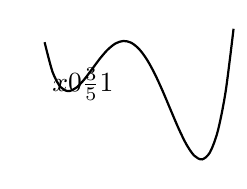
\begin{tikzpicture}
        \drawvec (-1, 0) -- (3, 0) node[below]{\(x\)};
        \draw[domain=-0.3:2.1, smooth, thick] plot (\x, {0.4*\x*\x*(5*\x - 6)*(\x - 2)});
        \fillpoint*{0, 0}[\(0\)][below];
        \fillpoint*{6/5, 0}[\(\frac{3}{5}\)][below left];
        \fillpoint*{2, 0}[\(1\)][below right];
    \end{tikzpicture}
\end{equation*}
Rozważmy na początek przedział otwarty \(\open{0}{1}\). Pochodna jest dodatnia w~przedziale \(\open{0}{\frac{3}{5}}\), dla \(x = \frac{3}{5}\) przyjmuje wartość \(0\), a~w~przedziale \(\open{\frac{3}{5}}{1}\) jest ujemna. Oznacza to, że funkcja \(P\) jest rosnąca w~przedziale \(\open{0}{\frac{3}{5}}\) i~malejąca w~przedziale \(\open{\frac{3}{5}}{1}\), więc dla \(x = \frac{3}{5}\) osiąga wartość największą dla przedziału \(\open{0}{1}\):
\begin{equation*}
    P\pars{\frac{3}{5}}
        = \frac{27}{125} \cdot \frac{4}{25}
        = \frac{108}{3125}
\end{equation*}
Jest to kandydat na wartość największą w~przedziale \(\closed{0}{1}\), ale trzeba jeszcze skontrolować, czy wartości przyjmowane na końcach tego przedziału domkniętego są mniejsze:
\begin{gather*}
    P\pars{0} = 0 \cdot \pars{1 - 0}^2 = 0 < \frac{108}{3125}\\
    P\pars{1} = 1 \cdot \pars{1 - 1}^2 = 1 \cdot 0 = 0 < \frac{108}{3125}
\end{gather*}
Zatem największą wartością prawdopodobieństwa \(P\) zdarzenia \(A \subset \Omega\) jest
\begin{equation*}
    P_\p{max} = P\pars{\frac{3}{5}} = \frac{108}{3125}
\end{equation*}
\subsubsection*{Zadanie~9.}
\begin{equation*}
    f\pars{x} = \frac{3x^2}{\underbrace{x^2 + 2x + 4}_{\Delta < 0 \implies \text{brak pierwiastków}}} \qquad x \in \real
\end{equation*}
Zauważmy, że
\begin{equation*}
    \limit[x \to \pm\infty] f\pars{x}
        = \limit[x \to \pm\infty] \frac{3x^2}{x^2 + 2x + 4}
        = 3
\end{equation*}
Obliczmy pochodną, aby zbadać przedziały monotoniczności funkcji:
\begin{equation*}
    \begin{split}
        f'\pars{x}
            &= \frac{\pars{3x^2}'\pars{x^2 + 2x + 4} - 3x^2\pars{x^2 + 2x + 4}'}{\pars{x^2 + 2x + 4}^2}
            = \frac{6x\pars{x^2 + 2x + 4} - 3x^2\pars{2x + 2}}{\pars{x^2 + 2x + 4}^2}
            = \frac{6x^3 + 12x^2 + 24x - 6x^3 - 6x^2}{\pars{x^2 + 2x + 4}^2}\\
            &= \frac{6x^2 + 24x}{\pars{x^2 + 2x + 4}^2}
            = \frac{6x\pars{x + 4}}{\pars{x^2 + 2x + 4}^2}
    \end{split}
\end{equation*}
Mianownik jest zawsze dodatni, więc znak pochodnej zależy tylko od licznika. Dlatego wykres znaku pochodnej wygląda następująco:
\begin{gather*}
    \upparabola{-4}{0}\\
    \tag{\(1\)} \forall x \in \open{-\infty}{-4}\colon f'\pars{x} > 0 \label{2020_11_06:9:first_increase}\\
    \tag{\(2\)} f'\pars{-4} = 0 \label{2020_11_06:9:first_zero}\\
    \tag{\(3\)} \forall x \in \open{-4}{0}\colon f'\pars{x} < 0 \label{2020_11_06:9:decrease}\\
    \tag{\(4\)} f'\pars{0} = 0 \label{2020_11_06:9:second_zero}\\
    \tag{\(5\)} \forall x \in \open{0}{+\infty}\colon f'\pars{x} > 0 \label{2020_11_06:9:second_increase}
\end{gather*}
Oznacza to, że
\begin{description}
    \item \(\mbox{(\ref{2020_11_06:9:first_increase})} \implies\) funkcja \(f\) jest rosnąca w~przedziale \(\open{-\infty}{-4}\)
    \item \(\mbox{(\ref{2020_11_06:9:first_increase})} \land \mbox{(\ref{2020_11_06:9:first_zero})} \implies \mbox{(\ref{2020_11_06:9:decrease})} \implies\) funkcja \(f\) osiąga w~punkcie \(x = -4\) osiąga maksimum lokalne:
        \begin{equation*}
            f\pars{-4} = \frac{48}{16 - 8 + 4}
                = 4
        \end{equation*}
    \item \(\mbox{(\ref{2020_11_06:9:decrease})} \implies\) funkcja \(f\) jest malejąca w~przedziale \(\open{-4}{0}\)
    \item \(\mbox{(\ref{2020_11_06:9:decrease})} \land \mbox{(\ref{2020_11_06:9:second_zero})} \land \mbox{(\ref{2020_11_06:9:second_increase})} \implies\) funkcja \(f\) osiąga w~punkcie \(x = 0\) osiąga minimum lokalne:
        \begin{equation*}
            f\pars{0} = 0
        \end{equation*}
    \item \(\mbox{(\ref{2020_11_06:9:second_increase})} \implies\) funkcja jest rosnąca w~przedziale \(\open{0}{+\infty}\)
\end{description}
Zatem wykres funkcji wygląda następująco:
\begin{mathfigure*}
    \drawcoordsystem{-8, -1}{8, 5};
    \draw[domain=-8:8, smooth, thick, ForestGreen, samples=70] plot (\x, {3*\x*\x/(\x*\x + 2*\x + 4)});
    \fillpoint*{-4, 4}[\(\pars{-4, 4}\)][above];
\end{mathfigure*}
\noindent
Zatem:
\begin{equation*}
    \set{f\pars{x} : x \in \real} = \closed{0}{4}
\end{equation*}
\subsubsection*{Zadanie~10.}
Zużycie najmniejszej ilości blachy oznacza zminimalizowanie pola powierzchni całkowitej puszki. Przyjmijmy, że \(r\) to promień podstawy puszki, a~\(h\) to jej wysokość. Objętość walca wyraża się wzorem:
\begin{gather*}
    V = \pi r^2h\\
    16\pi = \pi r^2h\\
    h = \frac{16}{r^2}
\end{gather*}
Pole powierzchni całkowitej walca to dwukrotność jego pola podstawy \(\pi r^2\) zsumowana z~polem powierzchni bocznej \(2\pi rh\) Zdefiniujmy funkcję pola powierzchni całkowitej walca w~zależności od \(r\):
\begin{equation*}
    S\pars{r}
        = 2\pi r^2 + 2\pi rh
        = 2\pi r^2 + 2\pi r \cdot \frac{16}{r^2}
        = 2\pi r^2 + 2\pi \cdot \frac{16}{r}
        = 2\pi\pars{r^2 + \frac{16}{r}} \qquad r \in \open{0}{+\infty}
\end{equation*}
Obliczmy jej pochodną:
\begin{equation*}
    S'\pars{r}
        = 2\pi\pars{2r - \frac{16}{r^2}}
        = 4\pi \cdot \frac{r^3 - 8}{r^2}
        = 4\pi \cdot \frac{\pars{r - 2}\overbrace{\pars{r^2 + 2r + 4}}^{\Delta < 0 \implies \text{brak pierwiastków}}}{r^2}
\end{equation*}
Wykres znaku pochodnej wygląda następująco:
\begin{equation*}
    \begin{tikzpicture}
        \drawvec (-2, 0) -- (2, 0) node[below]{\(r\)};
        \draw[thick] (-1.5, -1.5) -- (1.5, 1.5);
        \fillpoint*{0, 0}[\(2\)][below right];
    \end{tikzpicture}
\end{equation*}
Interesuje nas tylko przedział \(\open{0}{+\infty}\). W~przedziale \(\open{0}{2}\) pochodna jest ujemna, dla \(x = 2\), a~w~przedziale \(\open{2}{+\infty}\) jest dodatnia. Oznacza to, że funkcja \(S\) jest malejąca w~przedziale \(\open{0}{2}\) i~rosnąca w~przedziale \(\open{2}{+\infty}\), więc dla \(x = 2\) przyjmuje globalną wartość najmniejszą:
\begin{equation*}
    S_\p{min}
        = S\pars{2}
        = 2\pi\pars{4 + \frac{16}{2}}
        = 24\pi
\end{equation*}
Zatem najmniejsza ilość blachy, czyli \(24\pi\), jest potrzebna na puszkę o~promieniu \(r = 2\) i~wysokości \(h = 4\).
\subsubsection*{Zadanie~11.}
\begin{equation*}
    x^2 - 8x + k^2 + 4 = 0
\end{equation*}
Aby to równanie miało dwa pierwiastki (być może jako jeden podwójny), to \(\Delta\) musi być nieujemna
\begin{gather*}
    \Delta = 8^2 - 4 \cdot 1 \cdot \pars{k^2 + 4}\\
    64 - 4k^2 - 16 \geq 0\\
    48 - 4k^2 \geq 0\\
    4k^2 \leq 48\\
    k^2 \leq 12\\
    k \in \closed{-2\sqrt{3}}{2\sqrt{3}}
\end{gather*}
Jeśli oznaczymy pierwiastki równania przez \(x_1\) i~\(x_2\), to z~wzorów Viete'a mamy:
\begin{equation*}
    \frac{1}{x_1} + \frac{1}{x_2}
        = \frac{x_1 + x_2}{x_1x_2}
        = \frac{\frac{-\pars{-8}}{1}}{\frac{k^2 + 4}{1}}
        = \frac{8}{k^2 + 4}
\end{equation*}
Aby zminimalizować sumę pierwiastków, chcemy zmaksymalizować mianownik. To znaczy, że chcemy zmaksymalizować \(k^2\). Największe możliwe \(k^2\) to \(12\) przyjmowane dla \(k = \pm2\sqrt{3}\). Zatem najmniejsza możliwa suma pierwiastków to
\begin{equation*}
    \frac{8}{12 + 4} = \frac{8}{16} = \frac{1}{2}
\end{equation*}
\subsubsection*{Zadanie~12.}
Rozważmy przekrój osiowy tego stożka:
\begin{mathfigure*}
    \coordinate (A) at (-3, 0);
    \coordinate (B) at (3, 0);
    \coordinate (C) at (0, 7);
    \coordinate (S) at (0, 0);
    \drawrightangle{B--S--C};
    \draw (A) node[below left]{\(A\)}
        -- (B) node[below right]{\(B\)}
        -- node[above, sloped]{\(12\)} (C) node[above]{\(C\)}
        -- cycle;
    \draw[dashed] (C) -- node[right]{\(h\)} (S) node[below]{\(S\)};
    \path (S) -- node[below]{\(r\)} (B);
\end{mathfigure*}
Z~twierdzenia Pitagorasa mamy
\begin{gather*}
    r^2 + h^2 = 12^2\\
    r^2 = 144 - h^2\\
    r = \sqrt{144 - h^2}
\end{gather*}
Zdefiniujmy funkcję objętości tego stożka w~zależności od \(h\):
\begin{equation*}
    V\pars{h}
        = \frac{1}{3}\pi r^2h
        = \frac{1}{3}\pi\pars{144 - h^2}h
        = \frac{1}{3}\pi\pars{144h - h^3} \qquad h \in \open{0}{12}
\end{equation*}
Obliczmy pochodną tej funkcji:
\begin{equation*}
    V'\pars{h}
        = \frac{1}{3}\pi\pars{144 - 3h^2}
        = \pi\pars{48 - h^2}
        = \pi\pars{4\sqrt{3} + h}\pars{4\sqrt{3} - h}
\end{equation*}
Wykres pochodnej wygląda następująco:
\begin{equation*}
    \downparabola{-4\sqrt{3}}{4\sqrt{3}}[\(h\)]
\end{equation*}
Interesuje nas tylko przedział \(\open{0}{12}\). Pochodna jest dodatnia w~przedziale \(\open{0}{4\sqrt{3}}\), dla \(h = 4\sqrt{3}\) przyjmuje wartość \(0\), a~w~przedziale \(\open{4\sqrt{3}}{12}\) jest ujemna. Oznacza to, że funkcja \(V\) jest rosnąca w~przedziale \(\open{0}{4\sqrt{3}}\) i~malejąca w~przedziale \(\open{4\sqrt{3}}{12}\), więc dla \(h = 4\sqrt{3} \in \open{0}{12}\) przyjmuje globalną wartość najwększą:
\begin{equation*}
    V_\p{max} = V\pars{4\sqrt{3}} = \pi\pars{192\sqrt{3} - 64\sqrt{3}} = 128\pi\sqrt{3}
\end{equation*}
Zatem optymalny promień podstawy stożka wynosi \(4\sqrt{6}\), a~wysokość wynosi wtedy \(4\sqrt{3}\).
\subsubsection*{Zadanie~12.}
Zużycie możliwie najmniejszej ilości tektury jest równoważne zminimalizowaniu pola powierzchni całkowitej pudełka.
\begin{equation*}
    2\ell = 2\dm^3
\end{equation*}
Wszystkie wymiary w~rozwiązaniu tego zadania będziemy podawać odpowiednio w~\(\dm\), \(\dm^2\) i~\(\dm^3\). Oznaczmy przez \(a\) długość krawędzi podstawy, a~przez \(h\) oznaczmy wysokość prostopadłościanu:
\begin{gather*}
    2 = V = a^2h\\
    h = \frac{2}{a^2}
\end{gather*}
Zdefiniujmy funkcję pola powierzchni pudełka w~zależności od \(a\):
\begin{equation*}
    S\pars{a}
        = a^2 + 4ah
        = a^2 + 4a \cdot \frac{2}{a^2}
        = a^2 + \frac{8}{a} \qquad a \in \open{0}{+\infty}
\end{equation*}
Obliczmy pochodną tej funkcji:
\begin{equation*}
    S'\pars{a}
        = 2a - \frac{8}{a^2}
        = \frac{2a^3 - 8}{a^2}
        = \frac{2\pars{a - \sqrt[3]{4}}\overbrace{\pars{a^2 + a\sqrt[3]{4} + \sqrt[3]{16}}}^{\Delta < 0 \implies \text{ brak pierwiastków}}}{a^2}
\end{equation*}
Mianownik jest zawsze dodatni, więc znak pochodnej zależy tylko od licznika. Zatem wykres znaku pochodnej wygląda następująco:
\begin{equation*}
    \begin{tikzpicture}
        \drawvec (-2, 0) -- (2, 0) node[below]{\(a\)};
        \draw[thick] (-1.5, -1.5) -- (1.5, 1.5);
        \fillpoint*{0, 0}[\(\sqrt[3]{4}\)][below right];
    \end{tikzpicture}
\end{equation*}
Interesuje nas tylko przedział \(\open{0}{+\infty}\). Pochodna jest ujemna w~przedziale \(\open{0}{\sqrt[3]{4}}\), dla \(a = \sqrt[3]{4}\) przyjmuje wartość \(0\), a~w~przedziale \(\open{\sqrt[3]{4}}{+\infty}\) jest dodatnia. Oznacza to, że funkcja \(S\) jest malejąca w~przedziale \(\open{0}{\sqrt[3]{4}}\) i~rosnąca w~przedziale \(\open{\sqrt[3]{4}}{+\infty}\), więc dla \(a = \sqrt[3]{4}\) przyjmuje globalną wartość najmniejszą:
\begin{equation*}
    S\pars{\sqrt[3]{4}}
        = \sqrt[3]{16} + \frac{8}{\sqrt[3]{4}}
        = \frac{12}{\sqrt[3]{4}}
\end{equation*}
Krawędź podstawy powinna mieć długość \(a = \sqrt[3]{4}\), a~wysokość \(h = \frac{2}{\sqrt[3]{16}} = \frac{1}{\sqrt[3]{2}}\). Zużyjemy wtedy \(\frac{12}{\sqrt[3]{4}}\dm^2\) tektury.
